\documentclass[tikz,border=5pt]{standalone}
\usepackage[T1]{fontenc}
\usepackage{lmodern,amsmath,amssymb}
\usetikzlibrary{arrows.meta,calc,positioning,fit,backgrounds,shapes.geometric,matrix,decorations.pathreplacing,patterns}
\definecolor{ink}{gray}{0.08}
\definecolor{wash}{gray}{0.965}
\definecolor{soft}{gray}{0.45}
\tikzset{box/.style={draw=ink,line width=.65pt,fill=white,align=center,inner sep=4pt,outer sep=0pt,font=\small},flow/.style={draw=ink,line width=.65pt,-{Latex[length=1.8mm,width=1.3mm]},rounded corners=2pt},annotation/.style={font=\scriptsize,text=soft,align=center},groupbox/.style={draw=soft,dashed,line width=.45pt,fill=wash}}
\begin{document}
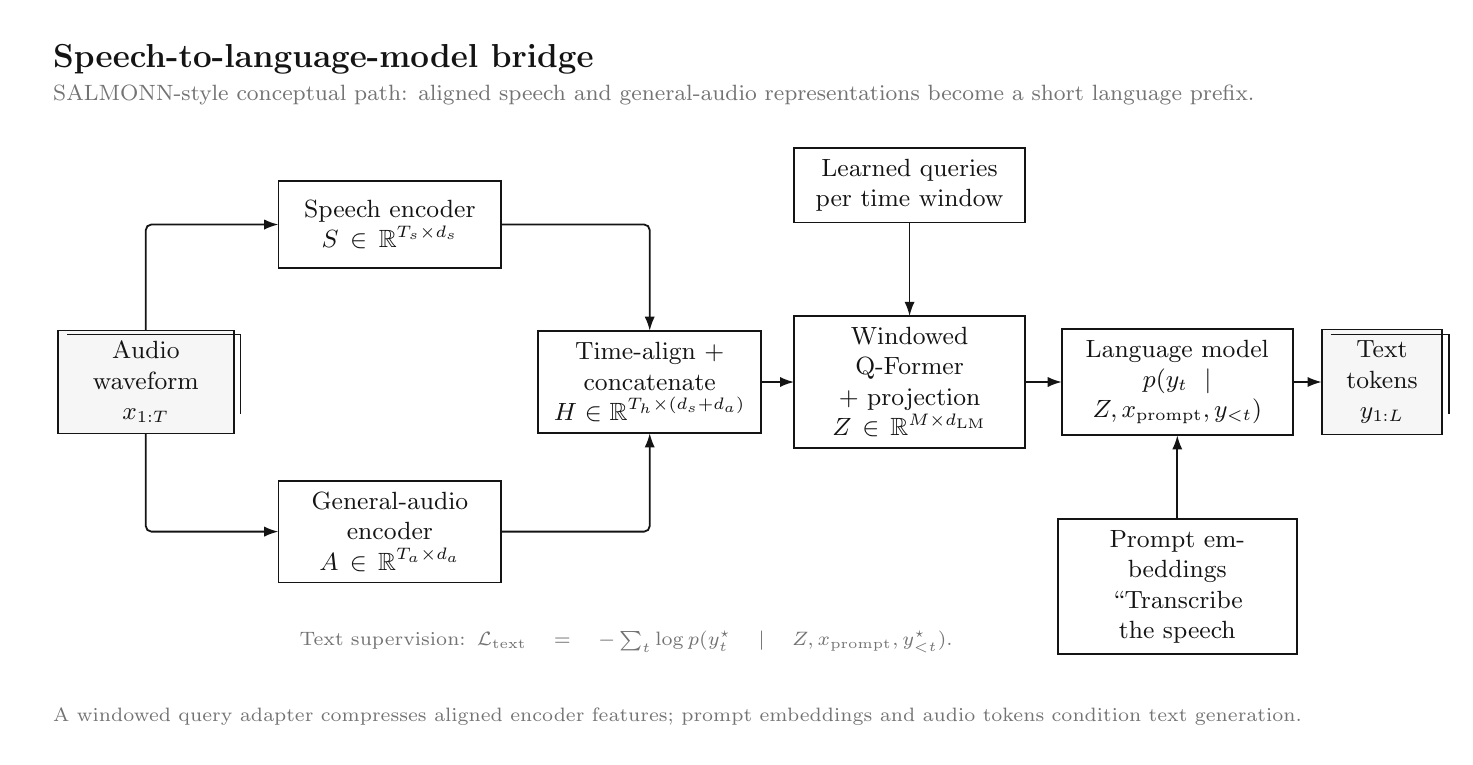
\begin{tikzpicture}[x=1cm,y=-1cm,font=\rmfamily,text=ink]

\path[use as bounding box] (0,0) rectangle (18,9);
\node[anchor=west,font=\large\bfseries] at (.2,.4) {Speech-to-language-model bridge};
\node[anchor=west,font=\footnotesize,text=soft] at (.2,.85) {SALMONN-style conceptual path: aligned speech and general-audio representations become a short language prefix.};
\begin{pgfonlayer}{background}
\end{pgfonlayer}
\node[box,fill=wash,minimum width=2.2cm,minimum height=1.0cm,text width=1.9500000000000002cm] (wave) at (1.5,4.5) {Audio waveform\\$x_{1:T}$};
\draw[ink,line width=.4pt] (0.4999999999999999,3.9) -- (2.7,3.9) -- (2.7,4.9);
\node[box,minimum width=2.8cm,minimum height=1.1cm,text width=2.55cm] (speech) at (4.6,2.5) {Speech encoder\\$S\in\mathbb{R}^{T_s\times d_s}$};
\node[box,minimum width=2.8cm,minimum height=1.1cm,text width=2.55cm] (sound) at (4.6,6.4) {General-audio encoder\\$A\in\mathbb{R}^{T_a\times d_a}$};
\node[box,minimum width=2.8cm,minimum height=1.3cm,text width=2.55cm] (align) at (7.9,4.5) {Time-align + concatenate\\$H\in\mathbb{R}^{T_h\times(d_s+d_a)}$};
\node[box,minimum width=2.9cm,minimum height=1.5cm,text width=2.65cm] (adapter) at (11.2,4.5) {Windowed Q-Former\\+ projection\\$Z\in\mathbb{R}^{M\times d_{\mathrm{LM}}}$};
\node[box,minimum width=2.9cm,minimum height=0.9cm,text width=2.65cm] (query) at (11.2,2.0) {Learned queries\\per time window};
\node[box,minimum width=2.9cm,minimum height=1.3cm,text width=2.65cm] (lm) at (14.6,4.5) {Language model\\$p(y_t\mid Z,x_{\mathrm{prompt}},y_{<t})$};
\node[box,minimum width=3.0cm,minimum height=1cm,text width=2.75cm] (prompt) at (14.6,7.1) {Prompt embeddings\\``Transcribe the speech};
\node[box,fill=wash,minimum width=1.5cm,minimum height=1cm,text width=1.25cm] (text) at (17.2,4.5) {Text tokens\\$y_{1:L}$};
\draw[ink,line width=.4pt] (16.55,3.9) -- (18.05,3.9) -- (18.05,4.9);
\begin{pgfonlayer}{background}
\draw[flow] (wave.north) -- (1.5,2.5) -- (speech.west);
\draw[flow] (wave.south) -- (1.5,6.4) -- (sound.west);
\draw[flow] (speech.east) -- (7.9,2.5) -- (align.north);
\draw[flow] (sound.east) -- (7.9,6.4) -- (align.south);
\draw[flow] (align.east) -- (adapter.west);
\draw[flow] (query.south) -- (adapter.north);
\draw[flow] (adapter.east) -- (lm.west);
\draw[flow] (prompt.north) -- (lm.south);
\draw[flow] (lm.east) -- (text.west);
\end{pgfonlayer}
\node[annotation,text width=12cm] at (7.6,7.8) {Text supervision: $\mathcal L_{\mathrm{text}}=-\sum_t\log p(y_t^{\star}\mid Z,x_{\mathrm{prompt}},y_{<t}^{\star})$.};
\node[anchor=west,align=left,font=\scriptsize,text=soft,text width=17.6cm] at (.2,8.75) {A windowed query adapter compresses aligned encoder features; prompt embeddings and audio tokens condition text generation.};
\end{tikzpicture}
\end{document}
